
\renewcommand{\EntradaBibtex}{ConteoLagartijas_UPV_2024}

\begin{frame}{\citetitle{\EntradaBibtex}$^*$ (1)}
\begin{block}{Motivacion} 
Las lagartijas (o flexiones) es un ejercicio muy completo que ofrece multiples beneficios para la salud, entre los mas importantes son: fortalecimiento muscular, mejorar la resistencia y la fuerza, aumenta la estabilidad, beneficiar a la salud osea y favorecer la movilidad y flexibilidad.
\begin{itemize}
\item Se implemento una aplicacion movil con retroalimentacion auditiva para contar lagartijas
\begin{itemize}
\item Permite al usuario llevar el conteo de las flexiones de manera facil
\end{itemize}
\end{itemize}
\end{block} 

\footfullcite*{\EntradaBibtex}
\end{frame}


\begin{frame}{\citetitle{\EntradaBibtex} (2)}
%\begin{block}{Pantallas Principales} 

%\begin{center}
%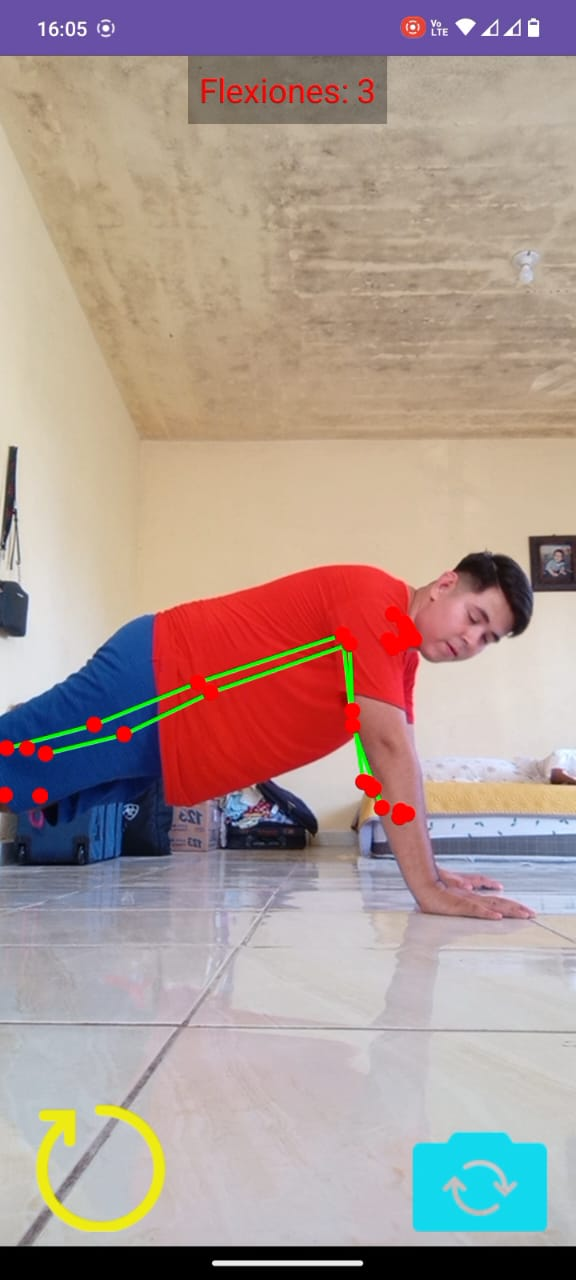
\includegraphics[width=0.40\linewidth]{2024_ConteoLagartijas/funcionamiento_app.png} 
%\end{center}


\begin{columns}
% Column 1
\column{.5\linewidth}



\begin{center}
	\begin{tabular}{cc}
		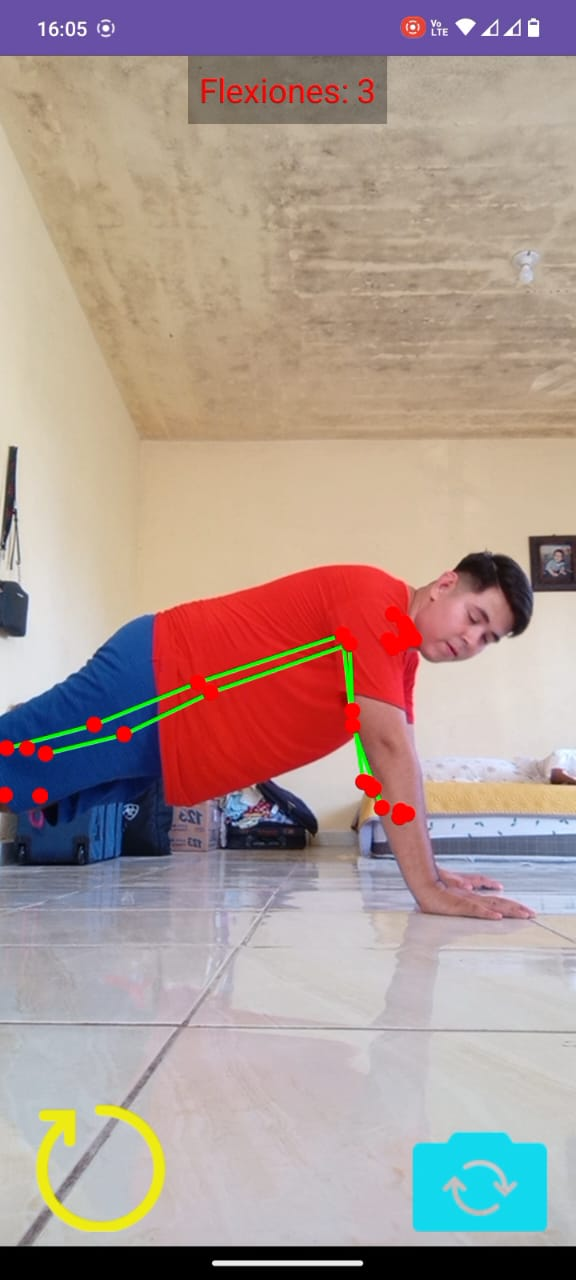
\includegraphics[width=0.40\linewidth]{2024_ConteoLagartijas/funcionamiento_app.png} &
		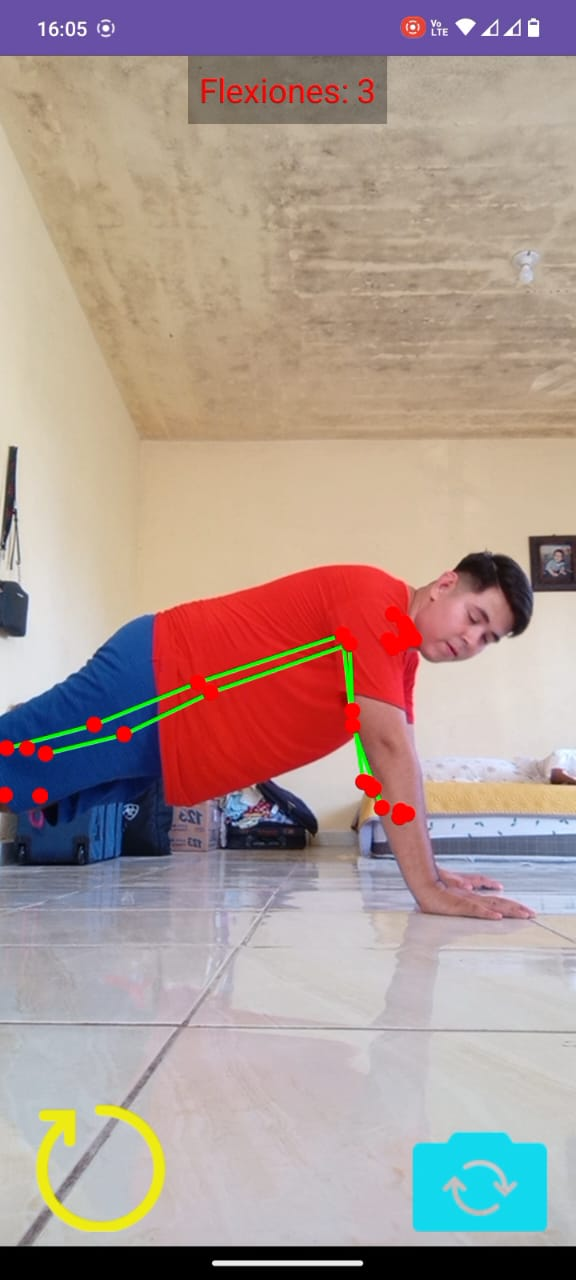
\includegraphics[width=0.40\linewidth]{2024_ConteoLagartijas/funcionamiento_app.png} \\
	\end{tabular}
\end{center}

\column{.5\linewidth}
\begin{center}
	\begin{tabular}{cccc}
		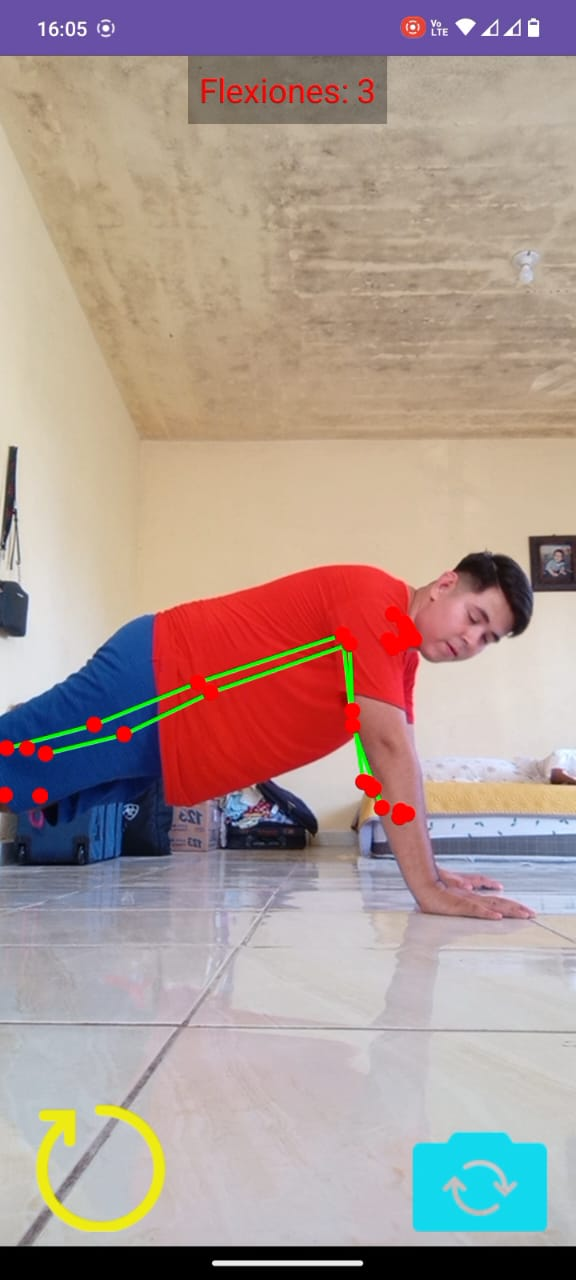
\includegraphics[width=0.40\linewidth]{2024_ConteoLagartijas/funcionamiento_app.png} &
 		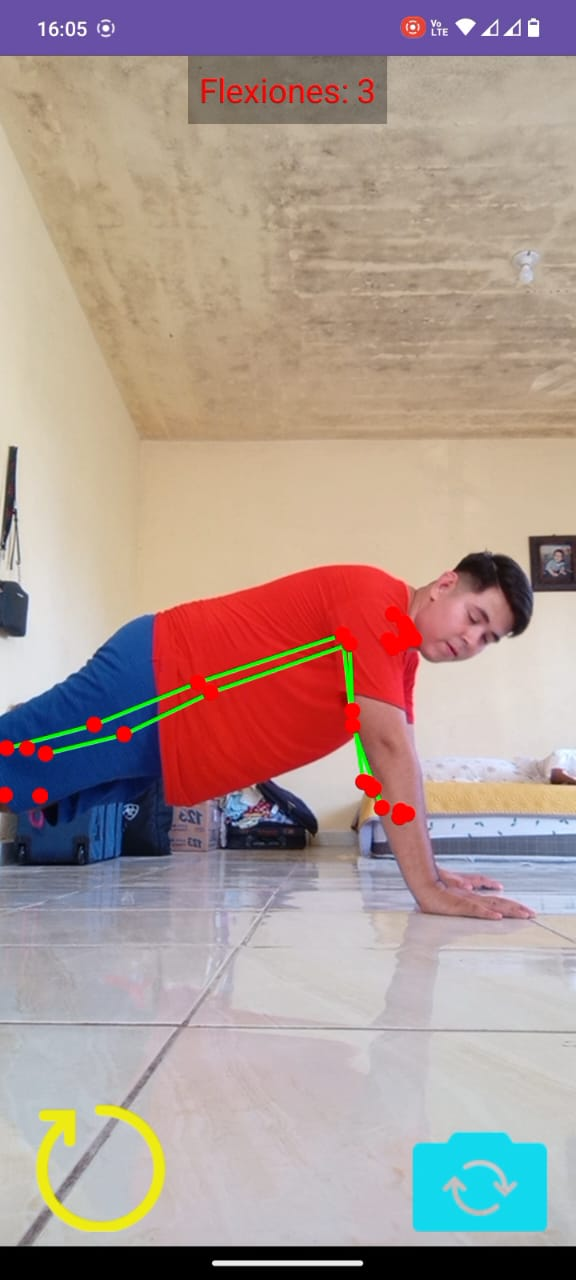
\includegraphics[width=0.40\linewidth]{2024_ConteoLagartijas/funcionamiento_app.png} \\
	\end{tabular}
\end{center}


\end{columns}

\end{frame}


